%%%%%%%%%%%%%%%%%%%%%%%%%%%%%%
% LATEX-TEMPLATE SAMENVATTING
%-------------------------------------------------------------------------------
% Voor informatie over het actief studeren en samenvatten, zie
% http://practicumav.nl/houding/studeren.html
% Voor readme en meest recente versie van het template, zie
% https://gitlab-fnwi.uva.nl/informatica/LaTeX-template.git
%
% Fouten bij het compileren in Overleaf? Check de README!
%%%%%%%%%%%%%%%%%%%%%%%%%%%%%%

%-------------------------------------------------------------------------------
%	PACKAGES EN DOCUMENT CONFIGURATIE
%-------------------------------------------------------------------------------

\documentclass[source]{uva-inf-article}
\usepackage[dutch]{babel}
% Packages voor tabel / mindmap
\usepackage{longtable}
\usepackage{tabu}
\usepackage{tikz}

\usetikzlibrary{mindmap,backgrounds}

%-------------------------------------------------------------------------------
%	GEGEVENS VOOR IN DE TITEL, HEADER EN FOOTER
%-------------------------------------------------------------------------------

% Vul de naam van de opdracht in.
\assignment{Naam van het samen te vatten boek}
% Vul het soort opdracht in.
\assignmenttype{Samenvatting}
% Vul de titel van de eindopdracht in.
\title{Titel van het document}

% Vul de volledige namen van alle auteurs in.
\authors{Auteur 1; Auteur 2}
% Vul de corresponderende UvAnetID's in.
\uvanetids{UvAnetID student 1; UvAnetID student 2}

% Vul altijd de naam in van diegene die het nakijkt, tutor of docent.
\tutor{Naam van de tutor}
% Voeg eventueel ook de naam van de docent of vakcoordinator toe.
\docent{}
% Vul hier de naam van de groep  in.
\group{Naam van de groep}
% Vul de naam van de cursus in.
\course{Naam van de (gekoppelde) cursus}
% Te vinden op onder andere Datanose.
\courseid{}

% Dit is de datum die op het document komt te staan. Standaard is dat vandaag.
\date{\today}

%-------------------------------------------------------------------------------
%	VOORPAGINA EN INHOUDSOPGAVE
%-------------------------------------------------------------------------------

\begin{document}
\maketitle

\tableofcontents

%-------------------------------------------------------------------------------
%	SAMENVATTINGEN
%-------------------------------------------------------------------------------

\lipsum[23]
% Je kunt een samenvatting opdelen in verschillende hoofdstukken, elk in een
% aparte file, en die importeren.
%\input{hoofdstuk}

%-------------------------------------------------------------------------------
%	VOORBEELD KOPPEN EN BIJLAGE
%-------------------------------------------------------------------------------

% De titel van het hoofdstuk
\section{Hoofdstuk X}
% De titel van de sectie / paragraaf uit het boek en de naam van de samenvatter.
% Hanteer dezelfde sectienummers als in het boek!

\subsection{Paragraaf zonder auteur}

\subsectionauthor[Voornaam Achternaam]{Paragraaf met auteur}

%-------------------------------------------------------------------------------
%	MIND MAP
%-------------------------------------------------------------------------------

\begin{figure}
\centering
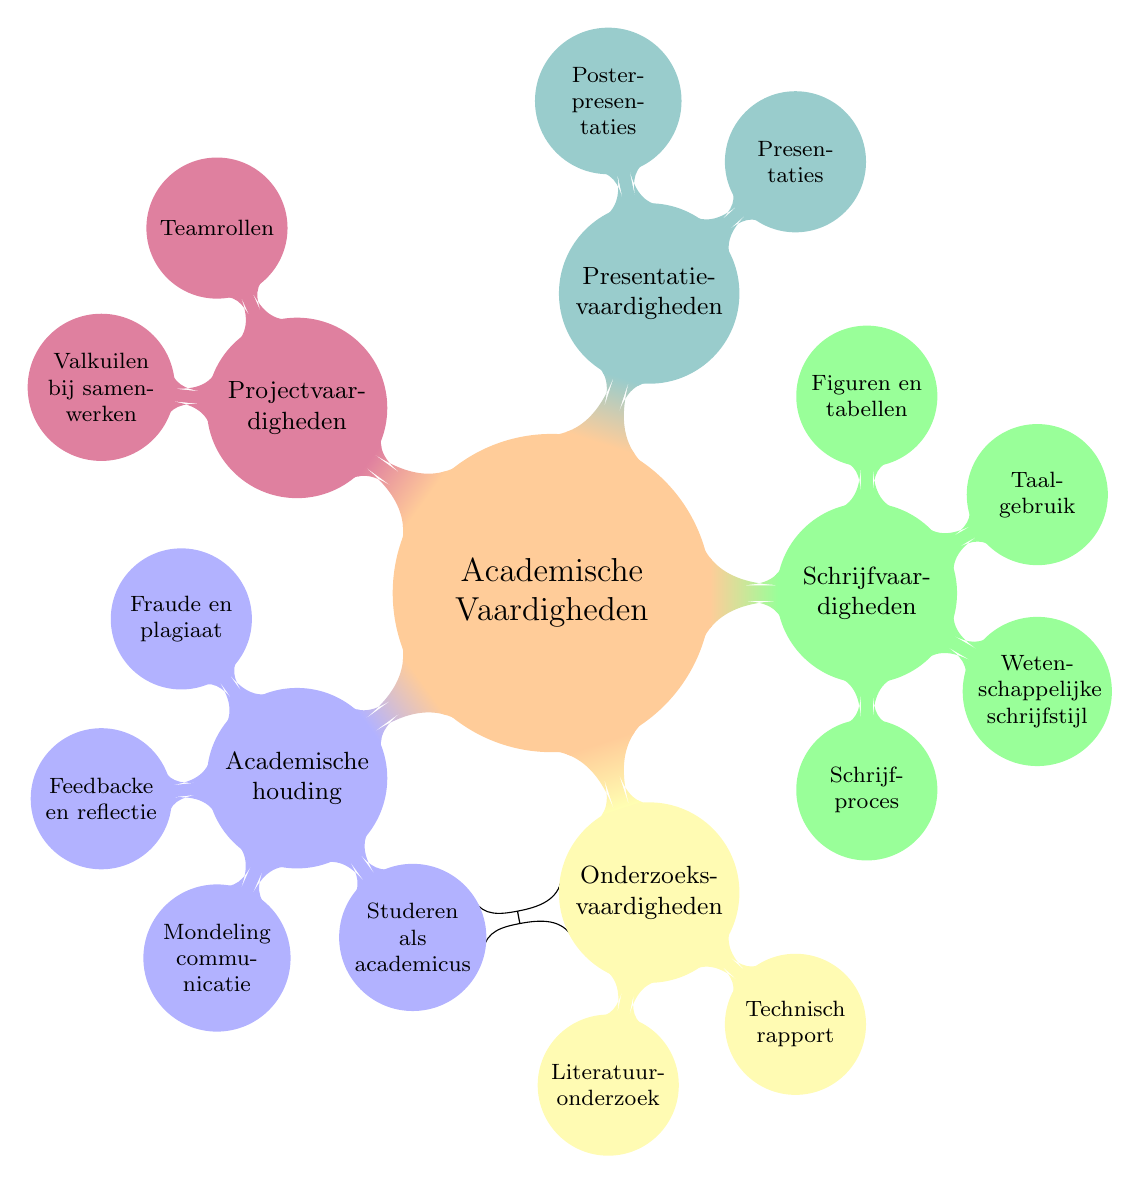
\begin{tikzpicture}[mindmap, grow cyclic, text width=2.7cm,
                    every node/.style=concept, concept color=orange!40,
    level 1/.append style={level distance=4.0cm,sibling angle=72},
    level 2/.append style={level distance=2.5cm,sibling angle=60},]

\node{Academische Vaardigheden}
    child [concept color=blue!30] { node {Academische houding}
	child { node {Fraude en plagiaat } }
	child { node {Feedbacke en reflectie } }
	child { node {Mondeling communicatie } }
	child { node (saa) {Studeren als academicus } }
    }
    child [concept color=yellow!30] { node (onv) {Onderzoeks-vaardigheden}
	child { node { Literatuur-onderzoek } }
	child { node { Technisch rapport } }
     }
    child [concept color=green!40] { node {Schrijfvaar-digheden}
	child { node { Schrijf-proces } }
	child { node { Weten-schappelijke schrijfstijl } }
	child { node { Taal-gebruik } }
	child { node { Figuren en tabellen } }
    }
    child [concept color=teal!40]{ node {Presentatie-vaardigheden}
	child { node { Presen-taties } }
	child { node { Poster-presen-taties } }
    }
    child [concept color=purple!50]{ node {Projectvaar-digheden}
	child { node { Teamrollen } }
	child { node { Valkuilen bij samenwerken } }
    };

\begin{pgfonlayer}{background}
    \draw [circle connection bar]
      (saa) edge (onv);
\end{pgfonlayer}

\end{tikzpicture}

\caption{Mindmap van de Academische Vaardigheden.}
\end{figure}

%-------------------------------------------------------------------------------
%	KOLOMMENSCHEMA
%-------------------------------------------------------------------------------

\begin{longtabu} to \linewidth {l|l|X|X}
\caption{Leeg kolomschema} \\
\rowfont\bfseries Hoofdzaak & Aspect & Inhoud & Voorbeeld \\ \hline
\endhead

\multicolumn{4}{r}{{Vervolgd op de volgende pagina}} \\
\endfoot

\endlastfoot

Hoofdzaak1
& Aspect1
& Inhoud1
& Voorbeeld1
\\ \cline{2-4}
& Aspect2
& Inhoud2
& Voorbeeld2 \\ \hline

Hoofdzaak2
& Aspect1
& Inhoud1
& Voorbeeld1
\\ \cline{2-4}

& Aspect2
& Inhoud2
& Voorbeeld2
\\ \hline

Hoofdzaak3
& Aspect1
& Inhoud1
& Voorbeeld1
\\ \cline{2-4}

& Aspect2
& Inhoud2
& Voorbeeld2
\\ \hline

\end{longtabu}
\end{document}
